\chapter{研究内容与方法}

\section{主要研究内容}
\begin{enumerate}
  \item 高温红外屏蔽复合材料的配方设计与理论筛选；
  \item 样品制备工艺参数优化（原料比例、烧结温度、保温时间）；
  \item 高温红外性能、抗氧化性能与微观结构表征；
  \item 建立性能指标与微结构参数的关联分析模型。
\end{enumerate}

\section{技术路线与方法}
项目采用“理论筛选-实验制备-高温测试-机制分析-反馈优化”的闭环路线：
\begin{enumerate}
  \item 通过文献与热力学判据初筛候选体系；
  \item 制备不同组分与工艺参数样品；
  \item 在目标温区测试 3--5\,$\mu$m 与 8--14\,$\mu$m 波段红外参数；
  \item 结合 XRD、SEM 等结果分析相组成与界面结构；
  \item 回代优化组分，形成稳定工艺方案。
\end{enumerate}

\begin{figure}[H]
\centering
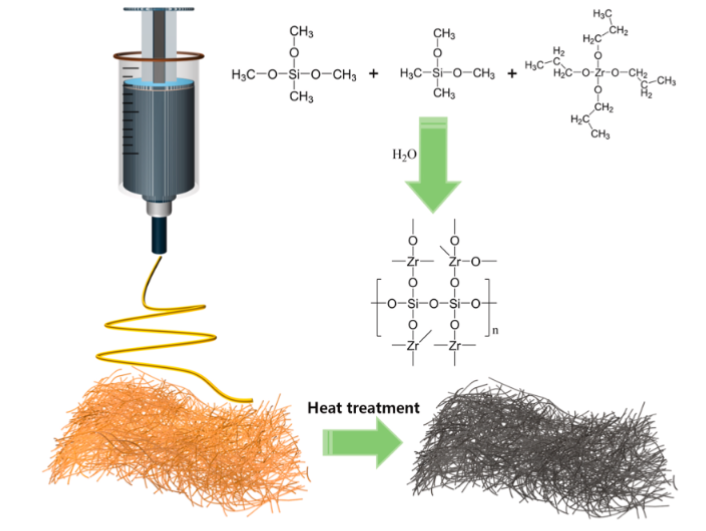
\includegraphics[width=0.88\textwidth]{picture/屏幕截图 2026-04-20 213515.png}
\caption{项目技术路线图}
\end{figure}

\section{实验条件}
\begin{itemize}
  \item 仪器设备：高温箱式炉、傅里叶红外光谱仪、XRD、SEM；
  \item 软件环境：Origin、MATLAB、jupyter（数据拟合与统计分析）；
  \item 样本来源：项目组自主制备样品。
\end{itemize}
